\chapter{Gestión de Proyectos}

Scrum es un marco de gestión de proyectos para el desarrollo incremental de productos, valiéndose de equipos autoorganizados. 



\subsection{Proyecto Scrum}

Un proyecto, en ingeniería de software, es un esfuerzo temporal que se lleva a cabo para crear un sistema, software o resultado único\footnote{Se parafrasea la definición del PMBOOK \cite{PMBOK-2004}.}. Los proyectos son organizados, en una empresa u organización, por el proceso de administración de proyectos. Según este proceso, el ciclo de vida de los proyectos se puede dividir en tres fases: inicio, ejecución y cierre (ver figura \ref{fig:PMIProject}). En la administración de proyectos es necesario planificar los proyectos y dicha actividad se suele hacer en la fase de inicio ("Starting phase" o "Project Start"). Pero, a diferencia de la metodología clásica (ver figura \ref{fig:PMIProject}) en que la planificación estaba siempre al inicio y el desarrollo en la fase de ejecución, en el marco Scrum la planificación se distribuye durante todo el ciclo de vida del proyecto y en la fase de ejecución se hace el desarrollo incremental de productos (por incrementos de producto) en iteraciones cortas (Sprint) donde cada iteración tiene su respectiva planificación (ver figura \ref{fig:ScrumProject}) y su incremento de producto, en caso de haberlo logrado.

\begin{figure}[h]
  \centering
  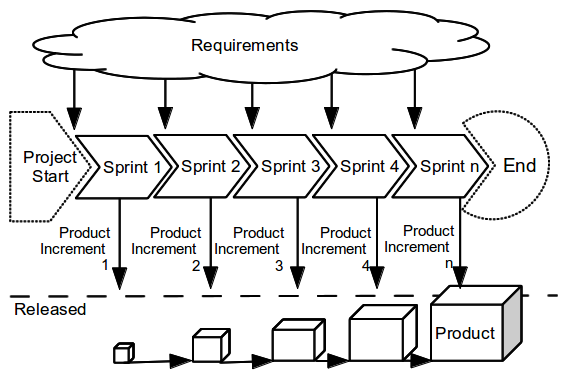
\includegraphics[width=0.90\textwidth]{ScrumProject}
  \caption{Proyecto Scrum}
  \centering
  \label{fig:ScrumProject} %\ref{fig:ScrumProject}
\end{figure}

Entonces podemos decir que en Scrum se piensa en muchos planes periódicos (a corto plazo). Los mismo pueden estar en un plan mayor a largo plazo pero de carácter flexible. También se puede realizar un plan global de entregables en base a los incrementos de producto estimado. Pero, desde esta perspectiva, hay que considerar que aunque se trabaje con planificaciones, los planes no son contratos a respetara a rajatabla.

%Triangle of Project Management
\subsection{Triángulo de la Gestión de proyectos}

El marco de Scrum cambia el triángulo clásico de la gestión de proyectos. El compromiso ya no es entre el tiempo, presupuesto y calidad; sino que se basa en el triángulo de: Presupuesto (Costo), Tiempo y funcionalidad (alcance) (ver figura \ref{fig:ScrumProjectManagementTriangle}). Además, tradicionalmente se ha intentado fijar el alcance para negociar y variar el presupuesto y el tiempo. En cambio, desde la agilidad, se intenta mantener fijos el tiempo y el presupuesto mientras se varía el alcance \cite{Martin-Alaimo-2014}.

\begin{figure}[h]
  \centering
  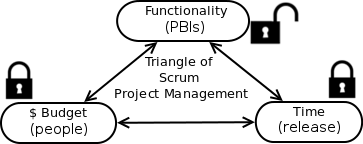
\includegraphics[width=0.80\textwidth]{ScrumProjectManagementTriangle}
  \caption{Triángulo de Gestión de Proyectos Scrum}
  \centering
  \label{fig:ScrumProjectManagementTriangle} %\ref{fig:ScrumProjectManagementTriangle}
\end{figure}

\subsection{Planificación de entregables}

Con esta metodología tampoco es necesario hacer una entrega final (o "releasing") ya que se pueden hacer entregas paulatinas. Para hacer entregas intermedias se puede crear un plan de muy alto nivel para múltiples Sprints durante una planificación de lanzamiento. Este plan de entregables o de de lanzamientos es una guía con la que se pretende reflejar las expectativas sobre las qué funciones se implementarán y cuando se completarán \cite{Scrum-Institute-2015}. También sirve como una base para monitorear el progreso dentro del proyecto. Pero siempre hay que considerar que no es un plan equivalente a un plan clásico, los ítos de releases no deberían ser compromisos rígidos y contractuales, y el desarrollo del proyecto no debería centrarse en respetar el plan. Por este motivo el plan de lanzamiento no es un plan estático. Pues, se cambia durante todo el proyecto cuando nuevos requerimientos o conocimientos están disponible y, por ejemplo, cuando entradas en el Scrum Product Backlog cambian y re-estiman. Por lo tanto este plan debe ser revisado y actualizado en intervalos regulares, por ejemplo, después de cada Sprint.

Para crear un plan de entregables se deben tener disponibles las siguientes cosas:

\begin{enumerate}
\item Un Product Backlog priorizado y estimado.
\item La velocidad estimada del Equipo Scrum.
\item Las condiciones de satisfacción (metas para la agenda, el alcance, los recursos)
\end{enumerate}

\subsection{Métricas}
Las métricas son indicadores que ayudan al equipo a medir su propio desempeño para poder hacer cambios basados en hechos. También es un soporte a la gestión de proyectos para poder medir el avance del proyecto, revisar la productividad y el desempeño de cada miembro del equipo y del propio equipo en su conjunto y poder hacer comparaciones entre diferentes equipos. Hay muchas métricas que nos pueden ser de utilidad, como por ejemplo las siguientes\footnote{Scott y Jeff \cite{Scott-Jeff-2013} y la  Scrumalliance en un artículo llamado "Velocity, How to Calculate and Use Velocity to Help Your Team and Your Projects", por Catia Oliveira (6 February 2014).}:

\begin{enumerate}

\item {\textbf{Velocity:} La 'velocidad'\footnote{"Sum of original estimates of all accepted work" \cite{Scott-Jeff-2013}.} es el número de unidades de trabajo o puntos de historia SP ("Story Points"\footnote{SP indica una cantidad de alcanse o trabajo que puede ser entregado o tamaño de producto estimado para entregar. Son la medida que representa la complejidad o esfuerzo necesario para terminar las tareas de una historia \cite{Jipson-Thomas-2015}.}) estimados y aceptados por un equipo en una iteración Sprint. En otras palabras, es el conjunto de puntos de historia totales conseguidos por el equipo al final de cada Sprint\footnote{\cite{Jipson-Thomas-2015}}.}

\item {\textbf{Average Velocity:} De la valocity de cada Sprint se calcula la velocidad promedio o "Average Velocity" que es el número de unidades de trabajo o SP promedio estimados y aceptados por un equipo en un conjunto de iteraciones Sprint. En un equipo ágil de velocidad estable, la velocidad promedio (de los últimos 4 Sprints) es un indicador adelantado de la velocidad estimada para el próximo Sprint (bajo las mismas condiciones de los Sprints usados para calcularla).}

\item {\textbf{Work Capacity:} La Capacidad es la suma de todos los trabajos reportados durante el Sprint, esten terminados o no\footnote{Scott y Jeff \cite{Scott-Jeff-2013}}. La capacidad es generalmente igual o superior a la Velocity. Aunque la Capacida puede, en raras ocasiones, caer por debajo de la velocidad. Esto se debe a que la velocidad se calcula en base a las estimaciones originales de trabajo, mientras que la capacidad se calcula en base a la suma de trabajo real reportado\footnote{Scott y Jeff \cite{Scott-Jeff-2013}}. Por lo que en el caso de que esto suceda, lo que indica es que el equipo ha sobre estimando la complejidad de los trabajos solicitados. También existen otras formas de calcular o entender la capacidad. Por ejemplo:

  \begin{enumerate}
  \item {\textbf{Capacidad en puntos ideales:} La capacidad puede ser una idealización basada en la velocidad promedio, o sea, los puntos de la historia que se pueden considerar gastar en la próxima carrera de velocidad.\footnote{\cite{Satish-Thatte-2013}}}

  \item {\textbf{Capacidad en horas:} La capacidad puede ser calculada en horas basados en la cantidad de miembros y la cantidad de horas efectivas de trabajo en un Sprint. Por ejemplo en un equipo de 8 miembros, con 6 horas de trabajo efectivo y un Sprint de 10 días, la capacidad en horas es igual a 480 hs (8 x 6 hs x 10).}

  \end{enumerate}

}

\item {\textbf{Focus Factor:} El Focus Factor es la relación entre la Velocity y la capacidad de trabajo: ( Velocity / Work Capacity ) x 100\%. La misma debe permanecer en la vecindad de 80 \% en promedio para un equipo saludable. Estos puntos de datos por debajo del 80 por ciento indican un equipo que está interrumpido o incapaz de convertir su trabajo estimado en trabajo aceptado mostrando poca previcibilidad. Cuando el valor es alto, cercano al 100, el equipo ha estado bajo la previsión de su capacidad pero esto no indica necesariamente que estan trabajando bien. Por ejemplo, el equipo puede estar aparentando ser perfecto forzando la coincidencia.}

\item {\textbf{Targeted Value Increase (TVI+)} El TVI+ responde a cuánto cambio ha habido en la velocidad del equipo a través del tiempo desde el primer Sprint. Es la Velocity del Sprint actual dividido la Velocity Original (velocity del primer sprint): ( Current Sprint’s Velocity / Original Velocity ) x 100\%. Sirve para medir el aumento de la contribución de valor de un equipo en base a su velocidad origen Sprint a Sprint.}

%\item \textbf{Percentage of Adopted Work}
%\item \textbf{Percentage of Found Work}
%\item \textbf{Accuracy of Estimation}
%\item \textbf{Accuracy of Forecast}
%\item \textbf{Targeted Value Increase (TVI+)}
%\item \textbf{Success at Scale}

\end{enumerate}
